\section{Background: Deterministic Execution}

Current deterministic execution systems \cite{liu_dthreads:_2011,merrifield_conversion:_2013,kai_lu_efficient_2014} allow an arbitrary multi-threaded program written in a conventional parallel programming language (like C or Java) to execute in a deterministic manner. The program's output and succession of internal states become solely a function of the program's explicit inputs and are unaffected by the nondeterministic interleaving of shared memory operations or OS scheduling decisions.

Determinism is achieved by keeping each thread's memory isolated from other threads', thereby converting a multi-threaded program into a collection of single-threaded programs, each of which are inherently deterministic. Periodically, threads are allowed to communicate with each other by \emph{retrieving} remote updates and \emph{committing} their local updates to make those updates available to remote threads. Previous systems have optimized the performance of this general approach along two main axes: 1) by increasing flexibility in when commits occur and 2) by reducing the number of remote threads that commits are made visible to (i.e., relaxing the memory consistency model).

\begin{figure}
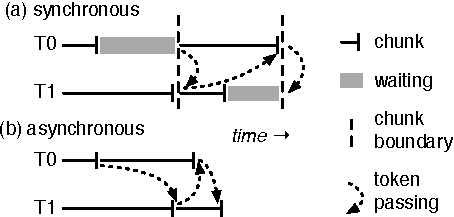
\includegraphics[width=3.0in]{figures/sync-async-chunks.pdf}
\caption{Synchronous versus asynchronous commit.}
\label{f:sync-async}
\end{figure}

Initial deterministic execution systems divided program execution into chunks consisting of a fixed number of instructions (typically 10-100,000) \cite{devietti_dmp:_2009,bergan_coredet:_2010,derek_r._hower_calvin:_2011} or separated by synchronization operations \cite{liu_dthreads:_2011}. 
After a thread executes one chunk it waits for all the other threads to execute their chunks before proceeding. This \emph{synchronous} approach (\autoref{f:sync-async}a) can lead to excessive waiting as threads often execute instructions or synchronization operations at different rates. An alternative \emph{asynchronous} approach was proposed by Merrifield and Eriksson \cite{merrifield_conversion:_2013} that eliminates global barriers, instead allowing threads to commit independently (\autoref{f:sync-async}b). In both synchronous and asynchronous approaches a global token circulates among threads in a deterministic round-robin order to ensure that commits occur deterministically.

\begin{figure}
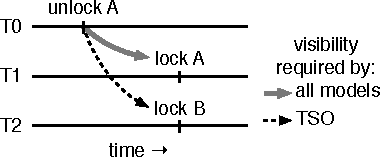
\includegraphics[width=3.0in]{figures/relaxed-consistency.pdf}
\caption{TSO requires that commits are global, while more relaxed models allow local commits that are visible to a subset of threads.}
\label{f:relaxed}
\end{figure}

Relaxing the consistency model improves the performance of determinism by making memory fences cheaper. Memory fence semantics define the number of threads to which commits must be made visible; with weaker consistency this number decreases which reduces the time it takes to push and pull commits. Consistency models like sequential consistency and total store order require that stores become visible in a total order that all threads agree on: commits must thus be a global operation (\autoref{f:relaxed}). Relaxed consistency models like DRF0 \cite{devietti_rcdc:_2011} and LRC \cite{kai_lu_efficient_2014} allow commits to be ``point-to-point'' with respect to a given synchronization object, i.e., the commit performed when releasing a lock need be visible only to the subsequent acquirer of that lock.

Removing global barriers and relaxing consistency offer orthogonal benefits and previous systems have explored these benefits both in isolation and in combination. \cite{merrifield_conversion:_2013} offers TSO with asynchronous commits, the RCDC system \cite{devietti_rcdc:_2011} adopts relaxed consistency but still uses synchronous commits, and RFDet \cite{kai_lu_efficient_2014} provides both asynchronous committing and relaxed consistency.

While RFDet could potentially provide the best performance of these schemes, the adoption of such an extremely relaxed\footnote{It is not obvious how further relaxations beyond LRC would be possible without breaking programming language semantics.} consistency model as LRC entails several additional costs. One concern is a space leak that arises from making commits visible only via a particular synchronization object. If a thread modifies some data and releases lock A, those modifications must be recorded until some other thread acquires lock A. This overhead is incurred for every lock release, causing space usage to scale with the number of lock objects. In the case that no other thread ever acquires lock A, space will be permanently leaked. This space overhead is not just a theoretical concern: in Section \ref{s:rfdet} we report large space overheads for RFDet on a benchmark with only a moderate number of synchronization operations.

 In addition to its space overheads, extremely weak consistency models like LRC are difficult for both humans \cite{adve_data_2010} and automated tools \cite{batty_mathematizing_2011,burckhardt_checkfence:_2007} to understand. The LRC model is substantially weaker than the most relaxed hardware consistency models (POWER and ARM) and thus programs compiled for a stronger model can break when executed on LRC. Recompilation with an LRC-aware compiler is necessary to generate the appropriate memory ordering instructions.

We propose that deterministic systems adopt stronger memory consistency models, such as the TSO model used in this work, to avoid these pitfalls. Next, we give an overview of the \lib system before discussing the optimizations that allow \lib to rival the performance of relaxed consistency approaches.

% We show that deterministic implementations of TSO can outperform weaker models because the cost of pushing and pulling commits can be quite low without resorting to weak consistency \ref{todo}. Furthermore, \textbf{the main performance bottleneck is the cost of deterministic synchronization} which requires centralized coordination in strong and weak consistency models alike. We show in \ref{todo} how to reduce the logical-physical clock skew that makes deterministic synchronization expensive. \TODO{may want to expand on clock skew here}

%%% Local Variables: 
%%% mode: latex
%%% TeX-master: "paper.tex"
%%% End:
